% IEEE conference format: US Letter, two columns, Times New Roman 10 pt body (24 pt title, 11 pt authors,
% 9 pt bold abstract, 8 pt captions/references), black text. Compile: tectonic paper/main.tex
% Numbers in this file that depend on the DP oracle come from numbers.tex, written by
% scripts/07_paper_assets.py; tables/ and figures/ are generated by the same script.
\documentclass[conference]{IEEEtran}
\usepackage{amsmath}
\usepackage{unicode-math}
% Body: Times New Roman (IEEE). It has no small-caps face, so section headings (small caps in the IEEE
% style) use the Times-metric TeX Gyre Termes; math uses its matching math font.
\setmainfont{Times New Roman}
\newfontfamily\scfont{texgyretermes-regular.otf}[RawFeature=+smcp]
\AtBeginDocument{\let\scshape\scfont}
\setmathfont{texgyretermes-math.otf}
\setmonofont{Courier New}[Scale=0.88]
\usepackage{graphicx,booktabs,array,balance}
\usepackage{tikz}
\usetikzlibrary{arrows.meta,positioning,calc}
% generated by scripts/07_paper_assets.py -- do not edit
\newcommand{\retrPzero}{0}
\newcommand{\fonePzero}{0.709}
\newcommand{\gapPzero}{-0.00}
\newcommand{\delayPzero}{nan}
\newcommand{\ftPzero}{nan}
\newcommand{\costPzero}{101.4}
\newcommand{\retrPone}{12}
\newcommand{\fonePone}{0.855}
\newcommand{\gapPone}{0.46}
\newcommand{\delayPone}{0.6}
\newcommand{\ftPone}{0.50}
\newcommand{\costPone}{16.6}
\newcommand{\retrPtwo}{49}
\newcommand{\fonePtwo}{0.868}
\newcommand{\gapPtwo}{0.01}
\newcommand{\delayPtwo}{0.0}
\newcommand{\ftPtwo}{0.92}
\newcommand{\costPtwo}{50.0}
\newcommand{\retrPeight}{6}
\newcommand{\fonePeight}{0.841}
\newcommand{\gapPeight}{0.58}
\newcommand{\delayPeight}{2.7}
\newcommand{\ftPeight}{0.00}
\newcommand{\costPeight}{15.5}
\newcommand{\retrPthree}{3.4}
\newcommand{\fonePthree}{0.825}
\newcommand{\gapPthree}{0.80}
\newcommand{\delayPthree}{5.8}
\newcommand{\ftPthree}{0.00}
\newcommand{\costPthree}{19.6}
\newcommand{\retrPfour}{4}
\newcommand{\fonePfour}{0.831}
\newcommand{\gapPfour}{0.61}
\newcommand{\delayPfour}{3.2}
\newcommand{\ftPfour}{0.00}
\newcommand{\costPfour}{16.0}
\newcommand{\retrPfourc}{5.4}
\newcommand{\fonePfourc}{0.842}
\newcommand{\gapPfourc}{0.26}
\newcommand{\delayPfourc}{2.1}
\newcommand{\ftPfourc}{0.00}
\newcommand{\costPfourc}{11.3}
\newcommand{\retrPfourchundred}{11}
\newcommand{\fonePfourchundred}{0.853}
\newcommand{\gapPfourchundred}{0.46}
\newcommand{\delayPfourchundred}{0.8}
\newcommand{\ftPfourchundred}{0.41}
\newcommand{\costPfourchundred}{15.0}
\newcommand{\retrPfourcthreehundred}{12.6}
\newcommand{\fonePfourcthreehundred}{0.856}
\newcommand{\gapPfourcthreehundred}{0.36}
\newcommand{\delayPfourcthreehundred}{0.5}
\newcommand{\ftPfourcthreehundred}{0.51}
\newcommand{\costPfourcthreehundred}{16.0}
\newcommand{\retrPfive}{6.8}
\newcommand{\fonePfive}{0.846}
\newcommand{\gapPfive}{0.30}
\newcommand{\delayPfive}{1.4}
\newcommand{\ftPfive}{0.00}
\newcommand{\costPfive}{12.0}
\newcommand{\gainweekly}{1.2}
\newcommand{\regPfourc}{1.7}
\newcommand{\regPfour}{6.3}
\newcommand{\regPthree}{10.0}
\newcommand{\regPone}{7.0}
\newcommand{\regPzero}{91.8}
\newcommand{\regPeriodic}{5.8}
\newcommand{\noracleseeds}{5}
\newcommand{\gapscope}{mean over 5 seeds}
\newcommand{\regPfourcHigh}{74}
\newcommand{\regPeriodicHigh}{37}
\newcommand{\regPfourcVeryHigh}{244}
\newcommand{\regPeriodicVeryHigh}{40}
\newcommand{\regRangeLo}{3}
\newcommand{\regRangeHi}{100}
\newcommand{\dpfour}{0.837}
\newcommand{\dptwelve}{0.859}
\newcommand{\pzeroref}{0.840}
\newcommand{\pzeromean}{0.709}
\newcommand{\pzeromin}{0.610}
\newcommand{\pzerowkNine}{0.823}
\newcommand{\pzerowkTen}{0.784}
\newcommand{\pzerowkEleven}{0.757}
\newcommand{\dweekNine}{1.8}
\newcommand{\dweekTen}{3.2}
\newcommand{\dweekEleven}{4.6}
\newcommand{\psvcone}{0.63}
\newcommand{\psvctwo}{0.52}
\newcommand{\psvcmed}{0.15}
\newcommand{\gtransrho}{0.77}
\newcommand{\gtruemean}{0.188}
\newcommand{\gpredmean}{0.104}
\newcommand{\gtransmae}{0.084}
\newcommand{\gtransbias}{-0.084}
\newcommand{\qfdayeight}{0.68}
\newcommand{\qfdaytwentyone}{0.63}
\newcommand{\qdrop}{0.004}
\newcommand{\qdroplo}{$-$0.001}
\newcommand{\qdrophi}{0.009}
\newcommand{\qfonePfour}{0.666}
\newcommand{\qfonePfourc}{0.666}
\newcommand{\qfonePfive}{0.684}
\newcommand{\qfonePzero}{0.651}


\begin{document}

\title{When to Retrain: Label-Free, Cost-Aware Drift Triage for Encrypted Traffic Classifiers}

\author{\IEEEauthorblockN{Lavnish J.}\IEEEauthorblockA{\textit{Reg.\ No.\ 24BCE2127}}
\and
\IEEEauthorblockN{Darsh S.}\IEEEauthorblockA{\textit{Reg.\ No.\ 24BDS0082}}
\and
\IEEEauthorblockN{Dhruv M.}\IEEEauthorblockA{\textit{Reg.\ No.\ 24BKT0116}}}

\maketitle

\begin{abstract}
A deployed encrypted-traffic classifier degrades as traffic drifts, yet ground-truth labels are unavailable after deployment and every retrain costs compute and labeling effort. We present a label-free, cost-aware triage layer that decides when a frozen classifier should be retrained. It fuses eight signals computed only from the classifier's probability output and raw input features into one drift score, removes weekly seasonality, detects persistent shifts with PELT, and prices the expected accuracy loss against the cost of retraining. A runtime-guarded label store refuses label access outside calibration and retraining. On a year of CESNET-TLS-Year22 traffic (50 services, five seeds) the score tracks true macro-F1 loss (Spearman 0.58; 0.85 after detrending). Our cumulative-cost rule reaches \fonePfourc{} macro-F1 with \retrPfourc{} retrains, against \fonePzero{} for never retraining and \fonePfour{} for the myopic rule, and lies \gapPfourc{} F1 points below the hindsight-optimal schedule at the same budget (\gapscope). On CESNET-QUIC22 it retrains on the day of the documented certificate change in all five seeds, while a fixed alarm threshold never fires.
\end{abstract}

\begin{IEEEkeywords}
encrypted traffic classification, concept drift, retraining policy, change-point detection, label-free monitoring
\end{IEEEkeywords}

\section{Introduction}
Operators classify encrypted traffic from what stays observable: packet sizes, timing, direction and flow-level statistics \cite{goli2018,alobaidy2019,rachmawati2021}. Models built on these features work well in the week they are trained. They do not stay accurate. Traffic drifts as applications update, certificates rotate and exporters change; in a month-long study of ISP QUIC traffic, classifiers trained on one week lost 9--13 accuracy points within three weeks \cite{luxemburk2023}. Restoring accuracy means retraining, which costs compute and, more importantly, fresh labels. For encrypted traffic the labels are the scarce resource. QUIC and Encrypted ClientHello remove the plaintext handshake fields earlier work used to label flows \cite{luxemburk2023,shamsimukhametov2022}, so an operator cannot cheaply grade a deployed model.

Two schedules dominate practice. Periodic retraining ignores the state of the traffic and spends labels whether or not the model has degraded; a fixed alarm threshold ignores what retraining costs \cite{gudepu2023}. Cost-optimal retraining has been formalized as a Markov decision process \cite{kanda2023}, but the detector in that formulation reads labels. The encrypted-traffic studies that measure drift \cite{kurapov2024,jancicka2024,malekghaini2023} stop short of saying when a measured shift justifies retraining, and Rachmawati et al.\ note the need for continuous updating while leaving its scheduling open \cite{rachmawati2021}.

We close this gap with a triage layer that sits beside a frozen classifier and decides, once per week and without labels, whether retraining is worth its price. Our contributions are:
\begin{itemize}
\item A \emph{label-free observer} that fuses eight signals from the classifier's probability output and raw inputs into one drift score, using sign orientation, family-balanced weights and per-generation baselines (Sec.~\ref{sec:observer}).
\item A \emph{cost-aware decision layer}: a frozen isotonic map from score to expected macro-F1 loss, a myopic rule that compares one week's expected loss with the fixed cost of a retrain, and a cumulative-cost rule that we introduce because the myopic rule cannot price a persistent, moderate loss (Sec.~\ref{sec:decision}).
\item An \emph{evaluation harness} with isolated policy timelines, an exact dynamic-programming bound on what any schedule achieves with hindsight, and three-layer enforcement that the decision path never reads labels (Secs.~\ref{sec:isolation} and~\ref{sec:setup}).
\item A \emph{full-year, five-seed evaluation} on CESNET-TLS-Year22 and a cross-protocol check on CESNET-QUIC22, with negative results reported next to positive ones (Sec.~\ref{sec:results}).
\end{itemize}

\section{Related Work}
\subsection{Encrypted traffic classification}
Port-based identification collapsed once applications adopted dynamic ports, and payload inspection is expensive, privacy-invasive and impossible on encrypted flows \cite{goli2018}. Machine learning on flow statistics and on packet size and timing sequences replaced it: decision trees on bidirectional flow features classify social-media applications \cite{alobaidy2019}, and deep models followed \cite{rachmawati2021}. Contextual TLS metadata identifies malware without decryption \cite{anderson2016}, while recent accuracy work centers on learned representations: ET-BERT pre-trains transformers on datagrams \cite{lin2022}, TFE-GNN fuses temporal graph structure \cite{zhang2023}, and MsETC learns multi-scale contrastive representations \cite{yang2024}. Encryption across TLS, HTTP/2 and QUIC changes which traffic characteristics an operator can observe at all \cite{akbari2021}. QUIC hides the handshake SNI, and recovering ground truth would need decryption infrastructure that operators judge infeasible at provider scale \cite{luxemburk2023}; neural classifiers degrade sharply once Encrypted ClientHello conceals the ClientHello \cite{shamsimukhametov2022}. This body of work improves the classifier. It does not say when a deployed one has stopped being trustworthy.

\subsection{Drift in traffic classification}
Drift in this domain is rapid, seasonal and class-dependent. Classifiers trained on one QUIC week lose 9--13 accuracy points by the third week, traced to a provider certificate change that altered early packet sizes \cite{luxemburk2023}. Anderson and McGrew show that distribution changes strongly affect malware classifiers trained on historical data \cite{anderson2017}. Malekghaini et al.\ measure drift across more than two years of ISP TLS data and find that the damage depends on the feature representation and the granularity of the task \cite{malekghaini2023}. Jan\v{c}i\v{c}ka et al.\ confirm a weekly seasonal component over a year of TLS traffic and observe that the features a classifier relies on most are disproportionately those that shift; they leave open how much change counts as meaningful \cite{jancicka2024}. Kurapov et al.\ conclude that monthly retraining suffices, but their data could not locate the point at which quality starts to degrade \cite{kurapov2024}. These two open questions are what a retraining trigger must answer.

\subsection{Label-free drift detection}
Jensen--Shannon divergence between traffic windows detects concept drift without labels and allows an earlier classifier to be reused \cite{yang2022}. Lughofer et al.\ track classifier confidence with a modified Page--Hinkley test \cite{lughofer2016}; Sethi and Kantardzic count samples that land in the classifier's margin of uncertainty and cut false alarms relative to detectors that watch only features \cite{sethi2017}; Souza et al.\ detect drift efficiently on high-speed streams with delayed or missing labels \cite{souza2020}. For change points, Aminikhanghahi et al.\ propose an unsupervised density-ratio detector with short delay \cite{aminikhanghahi2019}, and Smirnov shows that the penalty of PELT is a real optimization problem: small values raise false alarms, large values suppress detection \cite{smirnov2023}. These methods answer ``did something change?'' Whether the change justifies an expensive action lies outside their scope.

\subsection{Retraining policies and adaptation}
Gudepu et al.\ argue that fixed-threshold and periodic retraining are both inadequate and trigger retraining with an unsupervised outlier detector \cite{gudepu2023}. Kanda et al.\ model retraining under drift as a Markov decision process with explicit retraining and error costs and find detector-based policies cheaper than periodic ones, although their detector uses labels \cite{kanda2023}. Bagui et al.\ connect an Isolation Forest drift detector to incremental or full retraining on network-security data \cite{bagui2025}. Liu et al.\ ask for labels only on the most informative samples in an online active-learning framework \cite{liu2023oal}, and Cai et al.\ update encrypted-traffic classifiers incrementally with contrastive prototypes \cite{cai2024}; both still consume labels. LEAF shows in cellular networks that retraining can itself reduce accuracy and mitigates this with selective forgetting and oversampling \cite{liu2023leaf}. Li et al.\ match the adaptation strategy to the drift type \cite{li2024}, and Gama et al.\ survey the field \cite{gama2014}.

\subsection{Gap}
Encrypted-traffic studies establish that drift occurs \cite{luxemburk2023,kurapov2024,jancicka2024,malekghaini2023}. Label-free detectors show that it can be observed without labels \cite{yang2022,lughofer2016,sethi2017,souza2020}. Adaptive retraining beats static models \cite{gudepu2023,kanda2023,bagui2025,liu2023oal,cai2024}. What is missing is the decision between them: a label-free trigger, evaluated on encrypted traffic, that prices expected loss against retraining cost and is judged against the best schedule achievable with hindsight.

\section{Problem Setting}
A classifier $f_\theta$ is trained on labeled flows from an initial window W0 (weeks 1--2) and then frozen. Flows arrive in weekly batches $t=3,\dots,52$. At the end of week $t$ a policy returns \emph{retrain} or \emph{hold}; a retrain fits a new model on labels from the trailing $R=2$ weeks and deploys it for week $t{+}1$. The monitor sees only the probability matrix $P_t=f_\theta(x_t)\in\mathbb{R}^{n\times 50}$ and the raw features $x_t$. Labels are read in exactly two places: once, for the window that calibrates the loss map $g$, and at the moment a retrain fires. A policy is judged by mean weekly macro-F1, retrain count and cost.

\begin{figure*}[t]
\centering
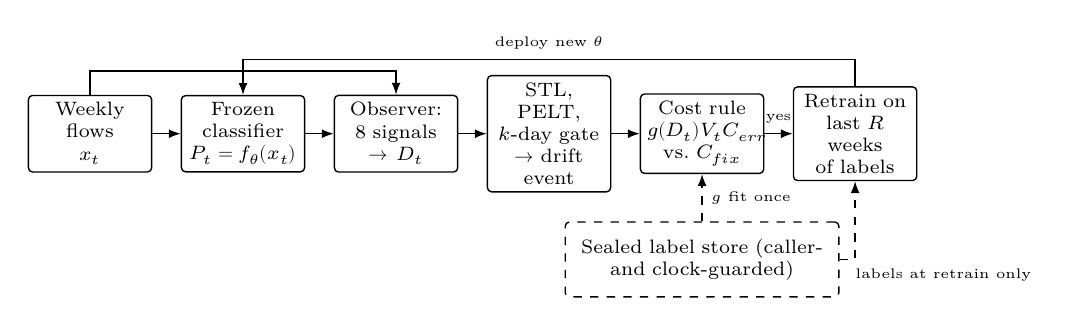
\begin{tikzpicture}[font=\scriptsize, node distance=0.36cm,
  box/.style={draw, rounded corners=1.5pt, minimum height=0.95cm, align=center, inner sep=2.5pt, line width=0.5pt, text width=1.05cm+3.4mm},
  arr/.style={-{Latex[length=1.5mm]}, line width=0.5pt}]
\node[box] (flow) {Weekly flows\\$x_t$};
\node[box, right=of flow] (clf) {Frozen\\classifier\\$P_t=f_\theta(x_t)$};
\node[box, right=of clf] (obs) {Observer:\\8 signals\\$\rightarrow D_t$};
\node[box, right=of obs] (det) {STL, PELT,\\$k$-day gate\\$\rightarrow$ drift event};
\node[box, right=of det] (cost) {Cost rule\\$g(D_t)V_tC_{err}$\\vs.\ $C_{fix}$};
\node[box, right=of cost] (ret) {Retrain on\\last $R$ weeks\\of labels};
\draw[arr] (flow) -- (clf); \draw[arr] (clf) -- (obs); \draw[arr] (obs) -- (det);
\draw[arr] (det) -- (cost); \draw[arr] (cost) -- node[above, font=\tiny]{yes} (ret);
\draw[arr] (flow.north) -- ++(0,0.3) -| (obs.north);
\draw[arr] (ret.north) -- ++(0,0.34) -| node[above, pos=0.25, font=\tiny]{deploy new $\theta$} (clf.north);
\node[box, dashed, below=0.6cm of cost, text width=3.3cm] (store) {Sealed label store (caller- and clock-guarded)};
\draw[arr, dashed] (store.east) -| node[below right, pos=0.2, font=\tiny]{labels at retrain only} (ret.south);
\draw[arr, dashed] (store.north) -- node[right, font=\tiny]{$g$ fit once} (cost.south);
\end{tikzpicture}
\caption{System overview. Everything left of the dashed store is label-free; labels flow only into the one-time calibration of $g$ and into a fired retrain.}
\label{fig:arch}
\end{figure*}

\section{Method}
\subsection{Label-free observer}\label{sec:observer}
For each day we compute eight signals from a sample of 10,000 flows: the mean and 10th-percentile maximum probability, the mean margin between the top two classes and the mean entropy of $P$; the Jensen--Shannon divergence between the predicted-class histogram and the reference histogram of the deployed model; the mean per-feature Kolmogorov--Smirnov statistic and an unbiased Gaussian-kernel $\mathrm{MMD}^2$ \cite{gretton2012} against a fixed reference sample (median-heuristic bandwidth); and the reject rate, the fraction of flows whose maximum probability falls below the 10th percentile of the reference.

Each signal enters with an orientation $\sigma_i\in\{-1,+1\}$ so that degradation always raises the score: maximum probability and margin fall under drift, while entropy, the divergences and the reject rate rise. Signals are centered on a per-generation baseline $b_i^{(m)}$, their value on a held-out fifth of generation $m$'s own training window at the daily sample size, and scaled by $\hat\sigma_i$, the robust (MAD) day-to-day spread of $s_i-b_i$ for the initial model over weeks 3--8, frozen thereafter. The composite is
\begin{equation}
D_t=\sum_i w_i\,\sigma_i\,\frac{s_i(t)-b_i^{(m)}}{\hat\sigma_i}.
\end{equation}
The hand-set weights give each of four families (confidence, prediction divergence, input drift, reject rate) a total weight of $1/4$; equal per-signal weights would hand the four collinear confidence statistics half the vote. Per-generation baselines keep $D$ comparable across retrains: it measures how far a model's inputs and outputs have moved from where they stood when that model was trained, in units of normal daily variation. Nothing in the score is learned.

\subsection{Conditioning and change detection}
The daily series of $D$ (eight missing calendar days are linearly interpolated) is deseasonalized with robust STL at period 7 \cite{cleveland1990}, keeping trend and residual; the day-of-week cycle is documented for this dataset \cite{jancicka2024}. We normalize with the median and MAD of the calm window (weeks 3--8) rather than a trailing window, because a trailing median acts as a high-pass filter and cancels a persistent step after half its length. PELT with an $\ell_2$ cost and minimum segment length 3 \cite{killick2012} finds change points within the current model's segment. The penalty is the smallest value on a logarithmic grid that yields no change point on the calm window ($\lambda=8$ here); the full sweep is logged, since the penalty trades false alarms against missed detections \cite{smirnov2023}. A change point becomes a \emph{drift event} only if the shift is upward, the next $k=3$ days stay above the pre-change mean, and the shift is still active today. The chain runs on the history seen so far, and a test that perturbs future observations confirms that past detections do not change.

\subsection{Cost-aware decision}\label{sec:decision}
Let $g$ map $D$ to expected macro-F1 loss. We fit $g$ once by isotonic regression on the days of weeks 3--10, using the true loss of the initial model (the only labeled reading outside retraining), and freeze it. Beyond the largest calibration score, $g$ continues with the non-negative least-squares slope instead of staying flat: a flat extension prices any drift larger than the calibration window at the window's maximum, and in a synthetic stress test it delayed the cumulative rule's first retrain from week 14 to week 17 after a shift at week 12. We did not run the flat variant on the real data. Let $V_t$ be the week's flow volume, $C_{err}$ the cost of one flow of macro-F1 loss, and $C_{fix}=C_{retrain}+C_{label}$. The \emph{myopic rule} (P4) retrains iff a drift event is active and
\begin{equation}
g(D_t)\,V_t\,C_{err} > C_{fix}.
\end{equation}
This compares a per-week loss rate with a one-off cost, so a persistent, moderate loss that stays just under the threshold is never corrected even though its cost grows without bound. The \emph{cumulative rule} (P4c) accumulates the excess loss since the current model was deployed,
\begin{equation}
A_t=\sum_{u=u_0}^{t}\max\bigl(0,\,g(D_u)-g_0\bigr)\,V_u\,C_{err},
\end{equation}
retrains once $A_t>C_{fix}$ and resets. The floor $g_0$ is the loss measured in the first week after the initial deployment (week 3), which no retrain removes because every model is deployed one week after its training data. Only the ratio $r=C_{err}V_{ref}/C_{fix}$ matters for decisions, with $V_{ref}$ the mean weekly volume in W0. It is the one operator-facing knob, and we sweep it over three orders of magnitude.

\subsection{Label isolation}\label{sec:isolation}
The label-free claim holds only if no label can reach the decision path, so we enforce it instead of relying on discipline. First, a static import-graph test fails if any module in the observer, detector, decision, classifier or replay packages reaches the label-bearing loader, harness or label store, directly or transitively and in every import form (\texttt{from pkg import module}, relative and \texttt{importlib}); the checker is itself mutation-tested against nine evasion patterns, and the form \texttt{from pkg import module} slips past a test that inspects only the module name of the import node. Second, the store checks its caller at runtime and refuses labels for any week after a simulation clock that only moves forward. Third, a behavioral test replaces the grader's output with random counts and verifies that the retrain decisions of P3, P4 and P4c stay identical while the oracle's change. Only the oracle P5, a non-competing upper bound, uses true performance.

\section{Experimental Setup}\label{sec:setup}
\subsection{Data}
CESNET-TLS-Year22 \cite{hynek2024} holds backbone TLS flows for all of 2022. We stream the public archive and keep a uniform Bernoulli sample of about 100,000 flows per day (the rate is stored, so true volumes are recoverable), then cap each replay day at 10,000 flows. Sampling is label-agnostic: a per-service cap would read labels on the operational stream and flatten the class prior that the divergence signal watches. The 50 services with the largest volume in W0 form a closed world; ranking by whole-year volume would use future information. Features are 60 flow statistics (bytes, packets and duration per direction, packet-sequence summaries, TCP flag counts, flow-end reasons and four 8-bin packet-size and inter-arrival histograms), log-transformed on count columns and standardized with a scaler fitted once on W0. The exporter update in week 10 changes packet-sequence data \cite{hynek2024}. Replay covers weeks 3--52, 50 decisions.

CESNET-QUIC22 \cite{luxemburk2023dib} spans 28 days, too few for weekly decisions, so we decide daily: W0 is days 1--7, replay covers days 8--28, STL is disabled and a retrain uses the last 7 days. The documented certificate change falls on day 22, in week 47 \cite{luxemburk2023}.

\subsection{Classifier, policies and metrics}
The substrate is a 100-round, 31-leaf LightGBM \cite{ke2017} with learning rate 0.1. With library defaults, 50-class training diverged on W0 (held-out accuracy 0.16 at a mean maximum probability of 0.9999); a hessian floor and L2 regularization, chosen on W0 alone, fix it (accuracy 0.845), and the trainer now fails loudly on that signature. A retrain fits at most 100,000 flows. We compare P0 never retraining; P1 and P2, periodic every 4 and 1 weeks; P3, an alarm when $D$ exceeds the calm median by three robust standard deviations; P4; P4c; and the oracle P5, which retrains when the deployed model's true loss exceeds 0.05. Each family's knob is swept: periodic $k\in\{1,2,3,4,6,8,13,26\}$, the P3 threshold, $r\in\{0.3,\dots,1000\}$ for P4 and P4c, and the P5 target. Costs are $C_{retrain}=100$ and $C_{label}=400$ in illustrative units; the default is $r=10$.

We report mean weekly macro-F1 over the 50 replay weeks and the retrain count. Cost is $\bigl[\sum_t\max(0,F_{ref}-F_t)V_tC_{err}\bigr]/C_{fix}+n_{retrain}$ in units of one retrain, where $F_{ref}$ is the initial model's held-out F1; clipping at zero matters, because an unclipped sum credits weeks above the reference and turns negative at large $r$. Detection delay counts weeks from the first week the deployed model's true loss exceeds 0.03 to the next retrain, and a retrain is a false trigger if the loss in its week is below 0.03. Because a retrained model depends only on its training week, the macro-F1 of every (generation, week) pair can be tabulated once, 1,275 pairs per seed, and dynamic programming then yields, for each retrain budget, the schedule with the highest mean F1 and, for each $r$, the schedule of minimum cost. We report each policy's \emph{gap}: that frontier at the policy's own budget and seed minus the policy's F1. Five seeds vary classifier randomness and subsampling, not the underlying traffic.

\begin{table*}[t]
\caption{Policy comparison on CESNET-TLS-Year22, default $r=10$. Mean over five seeds; $\pm$ is the standard deviation of macro-F1. Gap: points of macro-F1 below the DP-optimal schedule with the same number of retrains (\gapscope). Cost: units of one retrain, error cost clipped at zero. Delay in weeks; FT: false-trigger rate.}
\label{tab:main}
\centering\footnotesize
\begin{tabular}{@{}llrcrrrr@{}}
\toprule
 & Policy & Retrains & Macro-F1 & Gap & Cost & Delay & FT \\
\midrule
P0 & Never & 0.0 & 0.709 $\pm$ 0.002 & -0.00 & 101.4 & -- & -- \\
P1 & Periodic, $k{=}4$ & 12.0 & 0.855 $\pm$ 0.001 & 0.46 & 16.6 & 0.6 & 0.50 \\
P2 & Periodic, $k{=}1$ & 49.0 & 0.868 $\pm$ 0.000 & 0.01 & 50.0 & 0.0 & 0.92 \\
-- & Periodic, $k{=}8$ & 6.0 & 0.841 $\pm$ 0.000 & 0.58 & 15.5 & 2.7 & 0.00 \\
P3 & Threshold on $D$ & 3.4 & 0.825 $\pm$ 0.006 & 0.80 & 19.6 & 5.8 & 0.00 \\
P4 & Myopic cost rule & 4.0 & 0.831 $\pm$ 0.001 & 0.61 & 16.0 & 3.2 & 0.00 \\
P4c & Cumulative cost rule & 5.4 & 0.842 $\pm$ 0.002 & 0.26 & 11.3 & 2.1 & 0.00 \\
-- & Cumulative, $r{=}100$ & 11.0 & 0.853 $\pm$ 0.002 & 0.46 & 15.0 & 0.8 & 0.41 \\
P5 & Threshold oracle & 6.8 & 0.846 $\pm$ 0.001 & 0.30 & 12.0 & 1.4 & 0.00 \\
\bottomrule
\end{tabular}

\end{table*}

\section{Results}\label{sec:results}
\subsection{Drift, and whether $D$ tracks it}
Never retraining (P0) falls from a held-out F1 of \pzeroref{} to a weekly mean of \pzeromean{}, and to \pzeromin{} by week 52. The decline has two phases: a step at the week-10 exporter update (weekly F1 \pzerowkNine{} in week 9, \pzerowkTen{} in week 10, \pzerowkEleven{} in week 11), then slow erosion with a second drop after week 44. Antivirus services suffer most; \texttt{bitdefender-gravityzone} loses \psvcone{} F1 and \texttt{avast} \psvctwo{}, against a median loss of \psvcmed{} across the 50 services.

The label-free score tracks this loss. Across 50 weeks the Spearman correlation between weekly $D$ and true F1 loss is 0.58 (Pearson 0.86); after removing the linear trend from both series it is 0.85 (Pearson 0.94), and week-over-week changes correlate at 0.80. All clear the 0.3 gate we fixed before building the cost layer. A check over only the first 11 weeks, run while data was still downloading, gave 0.82; the full-year value is lower because $D$ stays high through the second half of the year while loss keeps growing. The signals are not equal (Table~\ref{tab:signals}). The confidence family and the reject rate carry the correlation (Spearman 0.67--0.73), JS divergence of predicted classes is nearly uninformative (0.05), and input drift is weak on ranks (KS 0.20, MMD 0.17). The composite correlates less than the reject rate alone (0.58 against 0.73) because the three weak signals dilute it. We did not ablate signals in the decision rules, so we cannot say whether a confidence-only score would also decide better.

\begin{table}[t]
\caption{Correlation of each oriented signal with true weekly macro-F1 loss of the never-retrained model (50 weeks).}
\label{tab:signals}
\centering\footnotesize
\begin{tabular}{@{}llcc@{}}
\toprule
Signal & Family & Spearman & Pearson \\
\midrule
Max. probability (mean) & Confidence & 0.70 & 0.87 \\
Max. probability (10th pct.) & Confidence & 0.72 & 0.87 \\
Top-2 margin (mean) & Confidence & 0.72 & 0.88 \\
Entropy (mean) & Confidence & 0.67 & 0.86 \\
JS divergence, predicted classes & Divergence & 0.05 & 0.32 \\
KS statistic (mean over features) & Input drift & 0.20 & 0.78 \\
MMD$^2$ & Input drift & 0.17 & 0.74 \\
Reject rate & Reject & 0.73 & 0.89 \\
\midrule
Composite $D$ & All & 0.58 & 0.86 \\
\bottomrule
\end{tabular}

\end{table}

\subsection{Policy comparison}
Table~\ref{tab:main} gives the default operating point. P4c retrains \retrPfourc{} times and lifts macro-F1 to \fonePfourc{}; the myopic rule P4 retrains \retrPfour{} times and reaches \fonePfour{}. P4c sits \gapPfourc{} points below the DP-optimal schedule at its budget and P4 \gapPfour{} (\gapscope), and P4c reacts in \delayPfourc{} weeks where P4 needs \delayPfour{}. Both fire in week 10, the exporter update, in all five seeds. The threshold rule P3 raises no false trigger but reacts \delayPthree{} weeks late on average and ends \gapPthree{} points below the frontier. Retraining every four weeks (P1) reaches \fonePone{} with \retrPone{} retrains and weekly retraining (P2) \fonePtwo{} with \retrPtwo{}, at false-trigger rates of \ftPone{} and \ftPtwo{}. The oracle P5, which reads true performance, sits \gapPfive{} points below the frontier: even an oracle with a fixed loss target is not optimal.

Against calendars the result is modest. At matched budgets the label-free rules and tuned periodic schedules land within a few tenths of a point of each other. Periodic retraining every 8 weeks uses \retrPeight{} retrains and reaches \fonePeight{}, \gapPeight{} points below the frontier; P4c uses \retrPfourc{} and reaches \fonePfourc{}, \gapPfourc{} below it. Near twelve retrains, retraining every four weeks (\fonePone{}, gap \gapPone{}) and P4c at $r=100$ (\fonePfourchundred{}, gap \gapPfourchundred{}) are indistinguishable. The periodic interval is chosen in hindsight on the evaluation year, whereas P4c at $r=10$ is not tuned on it, and of the policies in Table~\ref{tab:main} P4c has the lowest cost, below the oracle P5. What the triage layer adds is timing that follows the traffic (Sec.~\ref{sec:quic}), a shorter detection delay than the 8-week calendar (\delayPfourc{} against \delayPeight{} weeks), and a cost knob an operator can set without knowing the right interval in advance.

\begin{figure}[t]
\centering
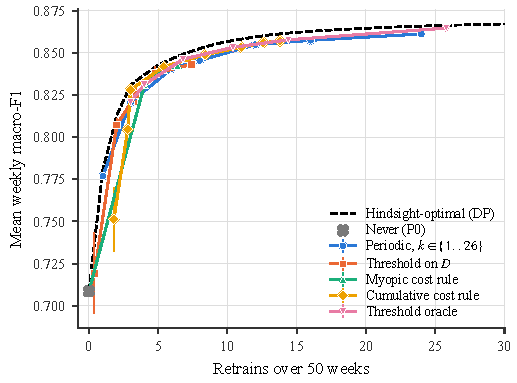
\includegraphics[width=\columnwidth]{figures/pareto}
\caption{Mean weekly macro-F1 against retrains for each policy family (markers: mean over five seeds; bars: standard deviation) and the DP-optimal frontier (dashed; \gapscope). Curves for P3, P4, P4c and P5 are traced by sweeping their knobs.}
\label{fig:pareto}
\end{figure}

\subsection{Distance from the optimal schedule}
Fig.~\ref{fig:pareto} places every family against the DP frontier (\gapscope). The frontier rises steeply to \dpfour{} at four retrains and reaches \dptwelve{} at twelve, so later retrains buy little. Every adaptive family and periodic retraining lie close to it, and none dominates. Weekly retraining gains \gainweekly{} points over P4c at $r=300$ (\retrPfourcthreehundred{} retrains, macro-F1 \fonePfourcthreehundred{}) for nearly four times the retrains. The two rules respond very differently to the knob (Table~\ref{tab:sweep}). At $r=3$ P4 never fires and stays at the macro-F1 of never retraining, while P4c with the same $g$ retrains 3.0 times; at high $r$ P4 saturates near 6.4 retrains while P4c keeps adapting. Inertness at low $r$ and saturation at high $r$ are the behaviors the cumulative rule was built to remove. In cost, measured as regret to the cost-optimal schedule at $r=10$ (\gapscope), P4c is \regPfourc{} retrain units above the optimum, P4 \regPfour{}, P3 \regPthree{}, never retraining \regPzero{}, and the best periodic interval, chosen in hindsight, \regPeriodic{}. P4c has the lowest regret of these policies only for $\regRangeLo\le r\le\regRangeHi$: at $r=300$ the hindsight-tuned calendar does better (\regPeriodicHigh{} against \regPfourcHigh{}), which fits the under-pricing of late-year loss by the frozen $g$ (Sec.~\ref{sec:disc}).

\begin{table}[t]
\caption{Cost-ratio sweep (five-seed means). Retrains, macro-F1 and gap in points.}
\label{tab:sweep}
\centering\footnotesize
\setlength{\tabcolsep}{3.2pt}
\begin{tabular}{@{}rrccrcc@{}}
\toprule
 & \multicolumn{3}{c}{P4 (myopic)} & \multicolumn{3}{c}{P4c (cumulative)} \\
\cmidrule(lr){2-4}\cmidrule(l){5-7}
$r$ & Ret. & F1 & Gap & Ret. & F1 & Gap \\
\midrule
0.3 & 0.0 & 0.709 & -0.00 & 1.8 & 0.751 & 5.54 \\
1 & 0.0 & 0.709 & -0.00 & 2.8 & 0.805 & 2.26 \\
3 & 0.0 & 0.709 & -0.00 & 3.0 & 0.828 & 0.26 \\
10 & 4.0 & 0.831 & 0.61 & 5.4 & 0.842 & 0.26 \\
30 & 5.4 & 0.840 & 0.43 & 8.4 & 0.849 & 0.46 \\
100 & 6.2 & 0.842 & 0.51 & 11.0 & 0.853 & 0.46 \\
300 & 6.4 & 0.842 & 0.55 & 12.6 & 0.856 & 0.36 \\
1000 & 6.4 & 0.842 & 0.55 & 13.8 & 0.857 & 0.34 \\
\bottomrule
\end{tabular}

\end{table}

\begin{figure*}[t]
\centering
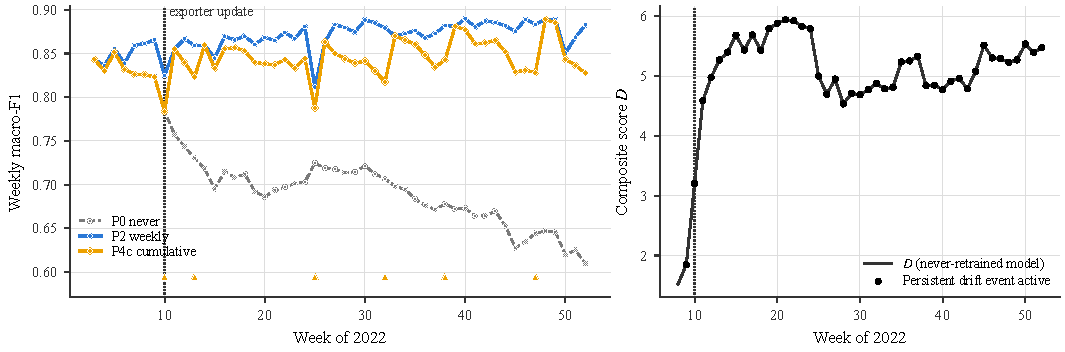
\includegraphics[width=\textwidth]{figures/timeline_tls}
\caption{CESNET-TLS-Year22, seed 0. Left: weekly macro-F1 for never retraining, weekly retraining and P4c; triangles mark P4c's retrains. Right: the composite score $D$ of the never-retrained model; dots mark weeks with an active persistent drift event. The dotted line is the week-10 exporter update.}
\label{fig:tls}
\end{figure*}

\subsection{Timing on TLS}
Fig.~\ref{fig:tls} shows the mechanism for seed 0. $D$ moves from \dweekNine{} to \dweekTen{} to \dweekEleven{} over weeks 9--11 as the exporter update takes hold; P4c retrains at the end of week 10 and weekly F1 recovers from 0.78 to 0.85. It retrains at weeks 13, 25, 32, 38 and 47 afterward. Week 25 is a one-week dip that even weekly retraining cannot avoid, since a model cannot be retrained on data it has not yet seen.

\subsection{Cross-protocol validation on QUIC}\label{sec:quic}
In all five seeds P4 and P4c retrain on day 22, the day of the documented certificate change, with no earlier retrain and zero detection delay, at the cost of one retrain; P3 never retrains (Table~\ref{tab:quic}). The periodic schedules retrain on days 11, 15, 19, 23 and 27 (every 4 days) or days 14 and 21 (every 7 days). The first brings a model that has seen the change one day after P4c does, after five retrains instead of one; the second retrains on day 21, a day too early to include any post-change data. Mean macro-F1 over the replay is \qfonePfour{} for P4, \qfonePfourc{} for P4c, \qfonePfive{} for P5 and \qfonePzero{} for never retraining (Fig.~\ref{fig:quic}).

\begin{table}[t]
\caption{CESNET-QUIC22: retrain days by seed (S0--S4). The documented certificate change is on day 22.}
\label{tab:quic}
\centering\footnotesize
\begin{tabular}{@{}lccccc@{}}
\toprule
 & S0 & S1 & S2 & S3 & S4 \\
\midrule
P3 threshold & -- & -- & -- & -- & -- \\
P4 myopic & 22 & 22 & 22 & 22 & 22 \\
P4c cumulative & 22 & 22 & 22 & 22 & 22 \\
P5 oracle & 10, 18 & 12 & 9, 14 & 10, 16 & 10, 15 \\
\midrule
Change point in $D$ & 12 & 11 & 11 & 12 & 11 \\
\bottomrule
\end{tabular}

\end{table}

\begin{figure}[t]
\centering
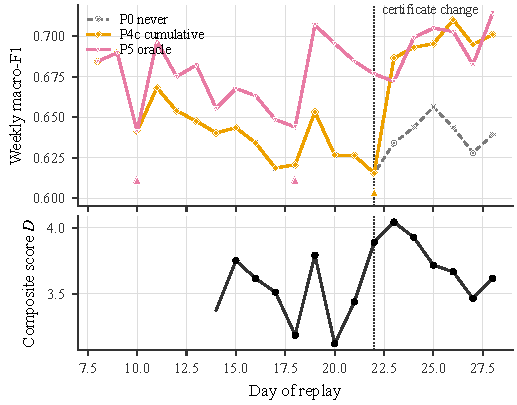
\includegraphics[width=\columnwidth]{figures/timeline_quic}
\caption{CESNET-QUIC22, seed 0 (decisions are daily). Top: macro-F1 of never retraining, P4c and the oracle; triangles mark retrains. Bottom: composite score $D$ of the never-retrained model. The dotted line is the documented certificate change on day 22.}
\label{fig:quic}
\end{figure}

The picture is less clean than a single step. The oracle retrains earlier, on days 9--18 depending on the seed, because the model had already lost accuracy before the change: never-retrained F1 falls from \qfdayeight{} on day 8 to \qfdaytwentyone{} on day 21 (seed 0), and a change point appears at day 11 or 12 in every seed. The simple F1 gap across day 22 is therefore small and noisy (mean \qdrop{}, range \qdroplo{} to \qdrophi{}), and we do not offer it as evidence; the timing match is. Two caveats apply. The five seeds share one physical event and one data sample, so 5/5 measures stability to classifier randomness, not five independent confirmations. And this check exposed a configuration-merge bug: the first run inherited the TLS exporter-event day (10) as the QUIC event day, which left decisions unchanged but produced an artificial 12-day delay and a pre/post gap of 0.043. Both are corrected above.

\section{Discussion and Limitations}\label{sec:disc}
Labels are not eliminated, only rationed. The loss map $g$ needs eight labeled weeks, which here include the exporter update, and a retrain needs two. In the late window (weeks 40--45), $g$ predicts a mean loss of \gpredmean{} where the never-retrained model's true loss is \gtruemean{}: it ranks days correctly (Spearman \gtransrho{}) but under-predicts the level by \gtransmae{}, so a map frozen in March underprices drift in November and biases both cost rules toward waiting. Recalibration is an obvious extension we did not test. The composite is carried by the confidence family, which is cheap to compute, and a confidence-only score would correlate better with loss than the composite does. The cost constants are illustrative and the fixed W0 reference makes absolute cost depend on the reference choice, which is why we lean on macro-F1 against retrains and on regret to the DP schedule. The experiments use sampled flows from one vantage point, a closed world of 50 services and weekly (TLS) or daily (QUIC) decisions; QUIC22 offers four weeks and one documented event. We have not studied partial retraining \cite{gama2014}, label-budgeted retraining \cite{liu2023oal} or open-world traffic.

\section{Conclusion}
A frozen encrypted-traffic classifier falls from \pzeroref{} to \pzeromin{} macro-F1 over a year, and a monitor that sees only its outputs and inputs can tell when. Our drift score correlates with true loss without reading a label, and a cumulative-cost rule converts it into retraining decisions that land near the best schedule hindsight allows, reach it without a tuned calendar, and fire on the day of a documented QUIC change that a fixed threshold misses. Calendars tuned in hindsight remain competitive at matched budgets, and most of the score's signal comes from classifier confidence. The pipeline, the label-isolation tests and the exact-optimum harness are at \texttt{github.com/Darsh2905/Label-free-retraining-triage}, so these comparisons can be repeated on other traffic and other drifts.

\balance
\bibliographystyle{IEEEtran}
\bibliography{refs}

\end{document}
